\section{1174031 - Muhammad Tomy Nur Maulidy}

\subsection{Teori}
\begin{enumerate}
\item Jelaskan dengan ilustrasi gambar sendiri apa perbedaan antara vanilla GAN dan cGAN\\
Perbedaan antara vanilla GAN dan CGAN terletak pada input proses suatu generator, pada vanilla GAN kita menggunakan data noise yang kemudian diproses menjadi suatu data fake atau palsu sedangkan pada cGAN kita menggunakan latent space atau label pada suatu generator. 
\begin{figure}[H]
	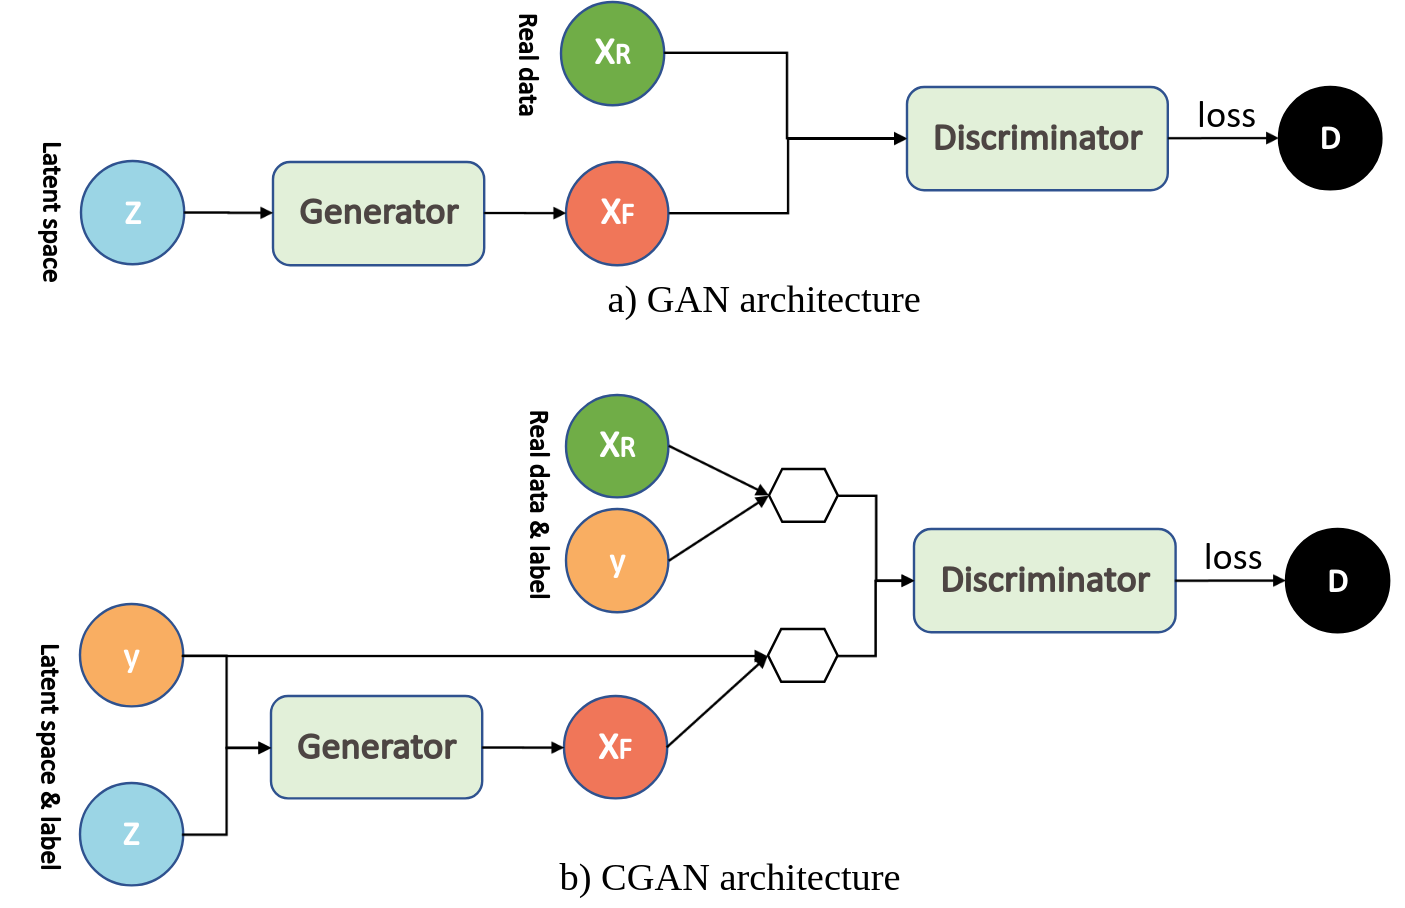
\includegraphics[width=4cm]{figures/1174031/9/1.png}
	\centering
	\caption{Vanilla GAN dan cGAN}
\end{figure}

\item Jelaskan dengan ilustrasi gambar sendiri arsitektur dari Age-cGAN\\
Pada Arsitektur Age-CGAN terdapat 4 bagian, yaitu : encoder, faceNet, generator dan discriminator.
untuk lebih jelasnya bisa dilihat pada ilustrasi gambar dibawah ini.
\begin{figure}[H]
	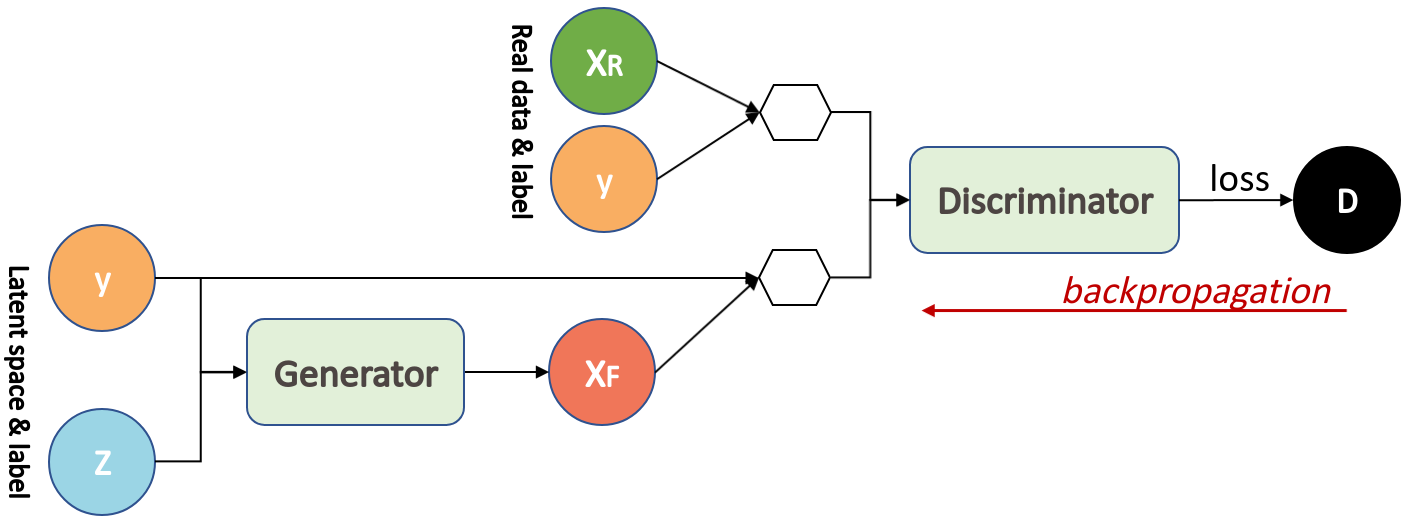
\includegraphics[width=4cm]{figures/1174031/9/2.png}
	\centering
	\caption{Arsitektur Age-cGAN}
\end{figure}

\item Jelaskan dengan ilustrasi gambar sendiri arsitektur encoder network dari Age-cGAN\\
Encoder mempelajari pemetaan terbalik dari gambar wajah input dan kondisi usia dengan vektor laten Z. jaringan encoder menghasilkan vektor laten dari gambar input.jaringan encoder adalah CNN yang mengambil gambar dari dimensi (64,64,3) dan mengubahnya menjadi vektor 100 dimensi. ada empat blok konvolusional dan dua lapisan padat. dan setiap blok konvolusional memiliki lapisan konvolusional, diikuti oleh lapisan normalisasi batch dan fungsi aktivasi kecuali lapisan konvolusional pertama.
\begin{figure}[H]
	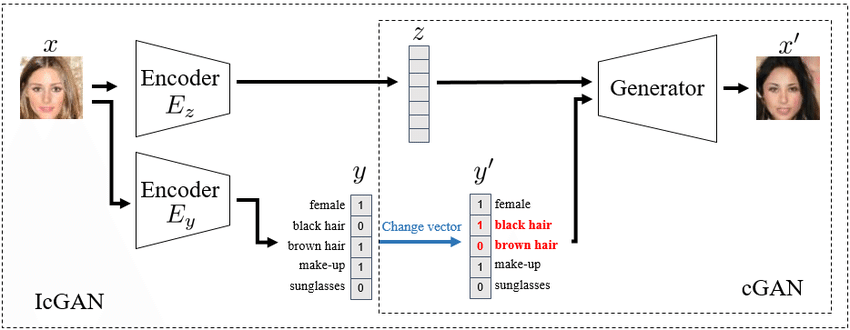
\includegraphics[width=4cm]{figures/1174031/9/3.png}
	\centering
	\caption{Arsitektur Encoder Network dari Age-cGAN}
\end{figure}

\item Jelaskan dengan ilustrasi gambar sendiri arsitektur generator network dari Age-cGAN\\
Pada generator dibutuhkan representasi tersembunyi dari gambar wajah dan vektor kondisi sebagai input dan menghasilkan gambar. generator adalah CNN dan dibutuhkan vektor laten 100 dimensi dan vektor kondisi y, dan mencoba menghasilkan gambar realistis dari dimensi (64,64,3). generator memiliki lapisan padat, membingungka dan konvlolusional. lalu dibutuhkan dua input satu adalah vektor noise dan yang kedua adalah vektor kondisi. vektor kondisi adalah informasi tambahan yang disediakan untuk jaringan. untuk Age-cGAN ini akan menjadi age.
\begin{figure}[H]
	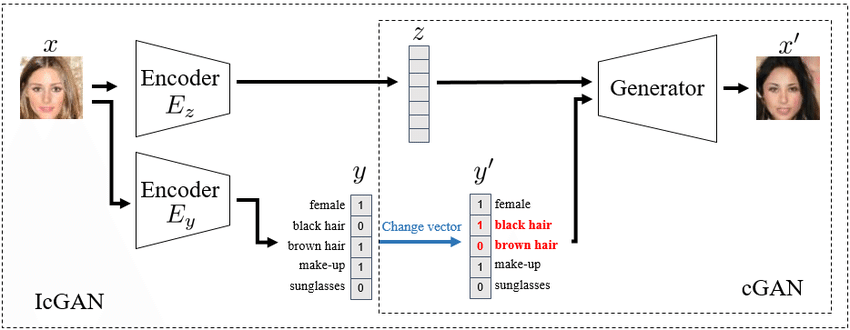
\includegraphics[width=4cm]{figures/1174031/9/3.png}
	\centering
	\caption{Arsitektur Generator Network dari Age-cGAN}
\end{figure}

\item Jelaskan dengan ilustrasi gambar arsitektur discriminator network dari
Age-cGAN\\
Diskriminator disini berfungsi untuk membedakan antara gambar asli dan gambar palsu. Diskriminator adalah CNN dan memprediksi gambar yang diberikan adalah nyata atau palsu. Disini terdapat blok konvolusional. Setiap blok konvolusional berisi lapisan konvolusional yang diikuti oleh lapisan normalisasi batch, dan fungsi aktifasi, kecuali blok konvolusional pertama, yang tidak memiliki normalisasi batch.
\begin{figure}[H]
	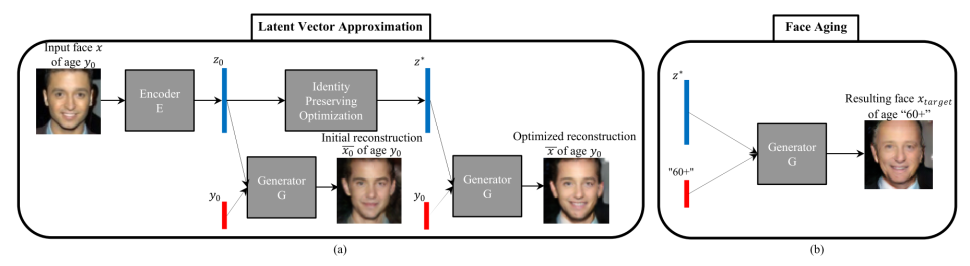
\includegraphics[width=4cm]{figures/1174031/9/4.png}
	\centering
	\caption{Arsitektur Discriminator Network dari Age-cGAN}
\end{figure}

\item Jelaskan dengan ilustrasi gambar sendiri apa itu apa itu pretrained Inception-ResNet-2 Model\\
Pretrained Inception-ResNet-2 Model adalah suatu model yang diciptakan untuk keperluan klasifikasi image dengan bobot di ImageNet.
\begin{figure}[H]
	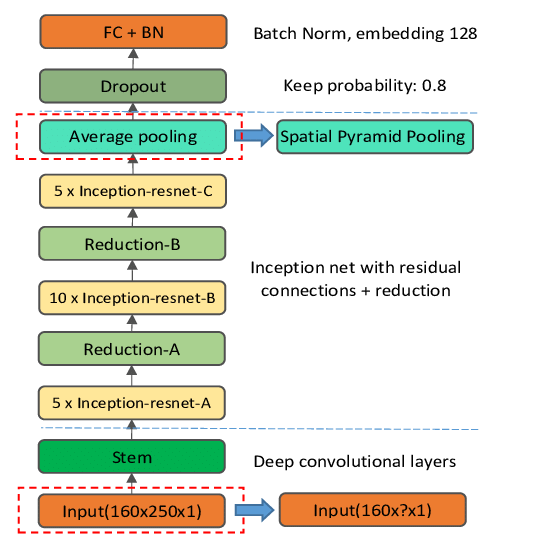
\includegraphics[width=4cm]{figures/1174031/9/5.png}
	\centering
	\caption{Pretrained Inception-ResNet-2 Model}
\end{figure}

\item Jelaskan dengan ilustrasi gambar arsitektur Face recognition network
Age-cGAN\\
FaceNet merupakan suatu jaringan pengenalan wajah yang mempelajari perbedaan antara gambar input x dan gambar yang direkonstruksi x. FaceNet ini dapat mengenali identitas seseorang dalam gambar yang diberikan. Model Inception, ResNet 50 atau Inception-ResNet-2 yang telah dilatih sebelumnya tanpa lapisan yang terhubung spenuhnya dapat digunakan. Embedding yang diekstraksi untuk gambar asli dan gambar yang direkonstruksi dapat dihitung dengan menghitung jarak Euclidean dari embeddings.
\begin{figure}[H]
	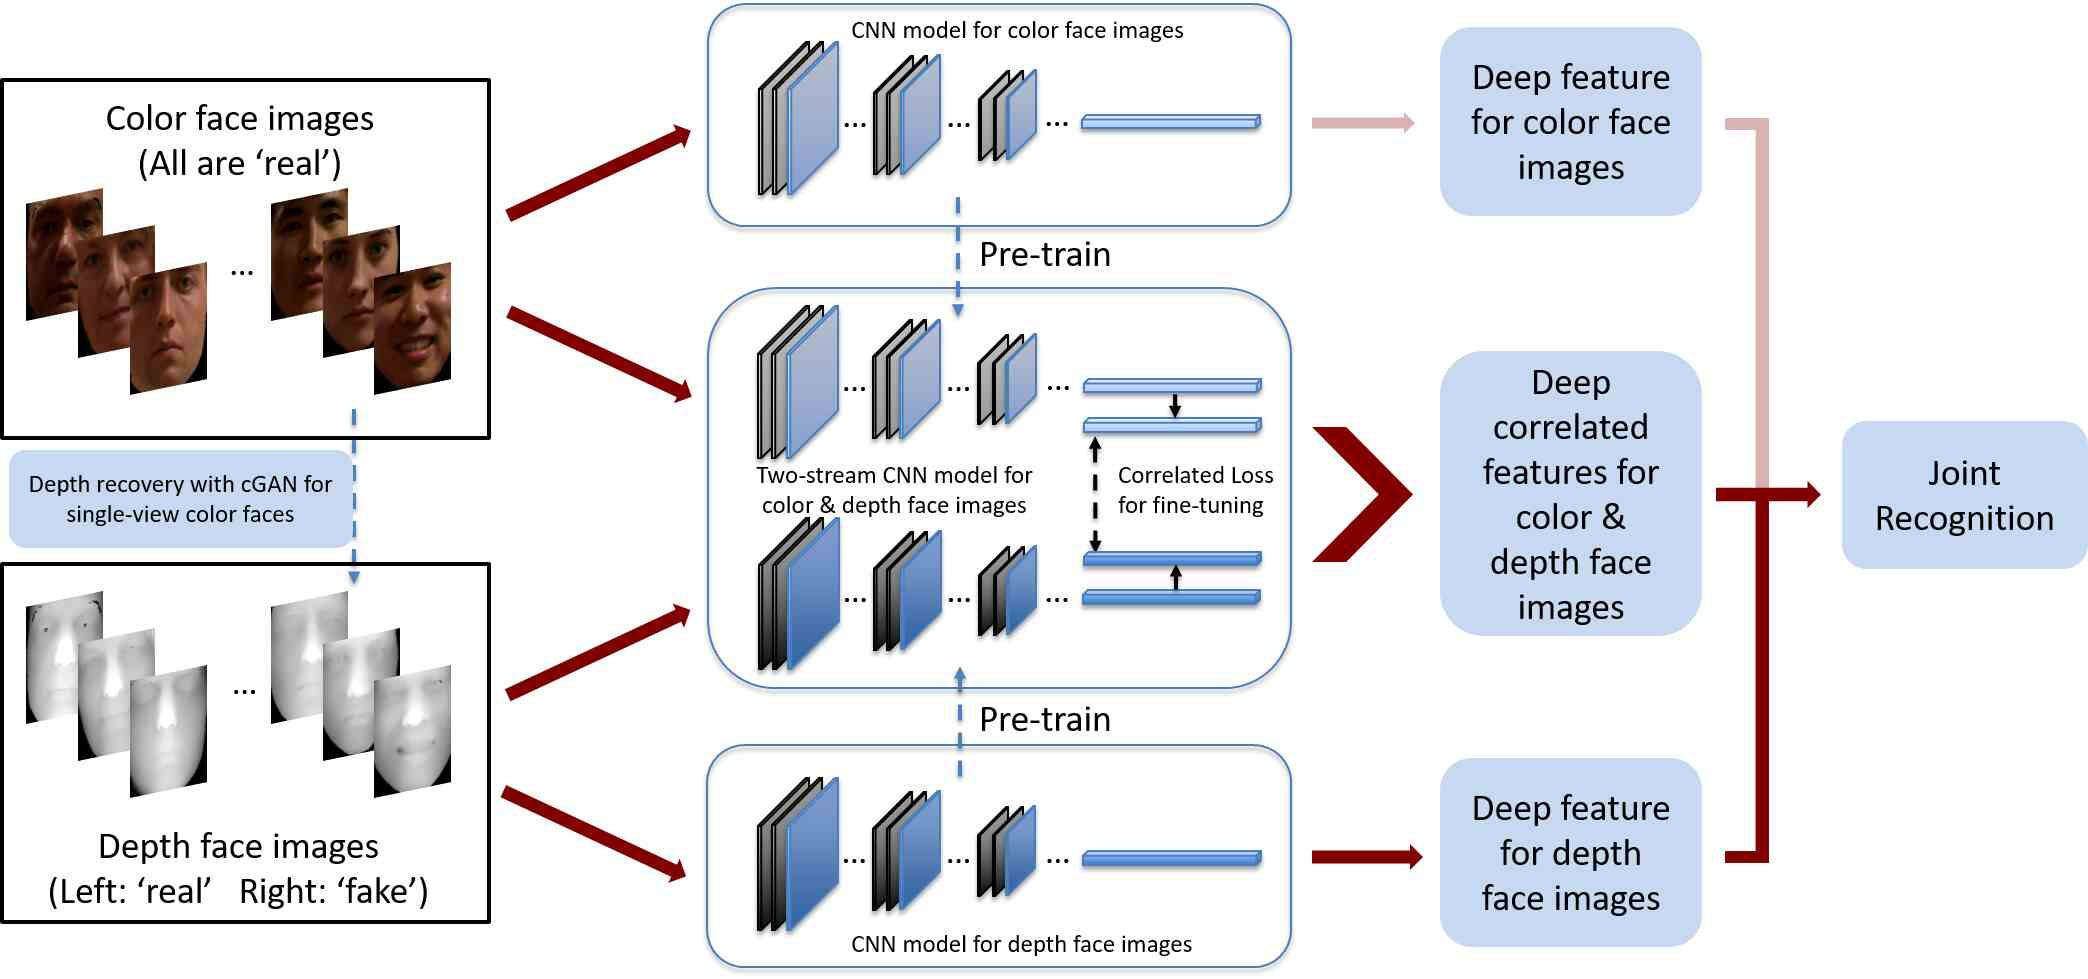
\includegraphics[width=4cm]{figures/1174031/9/6.png}
	\centering
	\caption{Arsitektur Face Recognition Network}
\end{figure}

\item Sebutkan dan jelaskan serta di sertai contoh-contoh tahapan dari Age-cGAN\\
Tahapan dari Age-cGAN adalah
\begin{itemize}
\item Input adalah semua data dan perintah yang dimasukkan yang kemudian nantinya akan diproses
\item Training, adalah suatu proses yang dimana data-data akan digunakan dalam proses training atau learning
\item Testing, adalah suatu proses yang melakukan evaluasi terhadap performa algoritma tersebut.
\end{itemize}

\item Berikan contoh perhitungan fungsi training objektif\\
Pada training network cGAn melibatkan fungsi optimalisasi. Melatih cGAN dapat dianggap sebagai permainan minimax, dimana generator dan diskriminator dilatih secara bersamaan. Dalam persamaan dibawah ini, a merupakan parameter dari jaringan generator, dan n mewakili parameter G dan D, logD(r) adalah kehilangan dalam model generator dan Pdata adalah distribusi dari semua gambar yang mungkin.
\begin{figure}[H]
	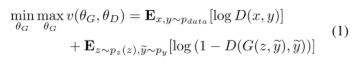
\includegraphics[width=4cm]{figures/1174031/9/7.png}
	\centering
	\caption{Perhitungan Fungsi Training Objektif}
\end{figure}

\item Berikan contoh dengan ilustrasi penjelasan dari Initial latent vector approximation\\
Initial latent vector approximation adalah suatu metode untuk memperkirakan vektor laten untuk mengoptimalkan  rekonstruksi gambar wajah. untuk memperkirakan vektor latent, kami memiliki jaringan pembuat encode. yaitu dengan melatih jaringan encoder pada gambar yang dihasilkan dan gambar nyata. setelah dilatih, jaringan encoder akan menghaslkan vektor laten dari distribusi bersandar. fungsi tujuan training untuk melatih jaringan encoder yaitu kehilangan jarak euclidean.

\item Berikan contoh perhitungan latent vector optimization\\
Selama optimasi vektor laten, dengan mengoptimalkan jaringan encoder dan jaringan generator secara bersamaan. persamaan yang kami gunakan untuk optimasi vektor laten adalah sebagai berikut :
\begin{figure}[H]
	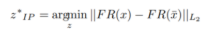
\includegraphics[width=4cm]{figures/1174031/9/8.png}
	\centering
	\caption{Perhitungan latent vector optimization}
\end{figure}
Pada persamaan diatas menunjukkan bahwa jarak euclidean antara gambar asli dan gambar yang direkonstruksi harus minimal. pada tahap ini, kita bisa mencoba meminimalkan jarak untuk memaksimalkan pelestarian identitas.

\end{enumerate}

\subsection{Praktek}
\begin{enumerate}
\item Nomor 1\\
\hfill\break
	\lstinputlisting[firstline=25, lastline=30]{src/1174031/9/1174031.py}
Pada kode diatas yaitu menghubungkan google drive dan mengextract dataset. adapun langkah-langkahnya bisa dilihat pada gambar berikut :
\begin{itemize}
\item Pertama, login terlebih dahulu ke akun google masing-masing dan masuk ke google colab
\item sambungkan google drive dengan google colab
\item Melakukan proses extract melalui notebook python di google colab. untuk mengestract bisa menggunakan codingan seperti pada kode diatas
\end{itemize}

\item Nomor 2\\
\hfill\break
	\lstinputlisting[firstline=33, lastline=57]{src/1174031/9/1174031.py}
Maksud dari kode diatas yaitu untuk melakukan load data dan melakukan fungsi perhitungan usia

\item Nomor 3\\
\hfill\break
	\lstinputlisting[firstline=60, lastline=99]{src/1174031/9/1174031.py}
Maksud encoder dalam kode diatas yaitu untuk mempelajari pemetaan terbalik dari gambar wajah yang diinput dan kondisi usia dengan vektor laten Z

\item Nomor 4\\
\hfill\break
	\lstinputlisting[firstline=102, lastline=140]{src/1174031/9/1174031.py}
Maksud generator dalam kode diatas yaitu generator network mampu bekerja dengan baik dengan membutuhkan representasi tersembunyi dari gambar wajah dan vektor kondisi sebagai input dan menghasilkan gambar

\item Nomor 5\\
\hfill\break
	\lstinputlisting[firstline=143, lastline=174]{src/1174031/9/1174031.py}
Maksud diskriminator pada kode diatas yaitu untuk membedakan antara gambar yang asli dan gambar yang palsu

\item Nomor 6\\
\hfill\break
	\lstinputlisting[firstline=177, lastline=309]{src/1174031/9/1174031.py}
Maksud dari kode diatas yaitu sebagai proses training dengan meload file.mat pada dataset, lalu kita melakukan epoch sebanyak 500 kali.

\item Nomor 7\\
\hfill\break
	\lstinputlisting[firstline=312, lastline=355]{src/1174031/9/1174031.py}
Maksud dari kode diatas yaitu dengan membuat model .h5 lalu meload data dengan menghasilkan result.

\end{enumerate}
